% Options for packages loaded elsewhere
\PassOptionsToPackage{unicode}{hyperref}
\PassOptionsToPackage{hyphens}{url}
\PassOptionsToPackage{dvipsnames,svgnames,x11names}{xcolor}
%
\documentclass[
]{report}

\usepackage{amsmath,amssymb}
\usepackage{iftex}
\ifPDFTeX
  \usepackage[T1]{fontenc}
  \usepackage[utf8]{inputenc}
  \usepackage{textcomp} % provide euro and other symbols
\else % if luatex or xetex
  \usepackage{unicode-math}
  \defaultfontfeatures{Scale=MatchLowercase}
  \defaultfontfeatures[\rmfamily]{Ligatures=TeX,Scale=1}
\fi
\usepackage{lmodern}
\ifPDFTeX\else  
    % xetex/luatex font selection
\fi
% Use upquote if available, for straight quotes in verbatim environments
\IfFileExists{upquote.sty}{\usepackage{upquote}}{}
\IfFileExists{microtype.sty}{% use microtype if available
  \usepackage[]{microtype}
  \UseMicrotypeSet[protrusion]{basicmath} % disable protrusion for tt fonts
}{}
\makeatletter
\@ifundefined{KOMAClassName}{% if non-KOMA class
  \IfFileExists{parskip.sty}{%
    \usepackage{parskip}
  }{% else
    \setlength{\parindent}{0pt}
    \setlength{\parskip}{6pt plus 2pt minus 1pt}}
}{% if KOMA class
  \KOMAoptions{parskip=half}}
\makeatother
\usepackage{xcolor}
\setlength{\emergencystretch}{3em} % prevent overfull lines
\setcounter{secnumdepth}{5}
% Make \paragraph and \subparagraph free-standing
\makeatletter
\ifx\paragraph\undefined\else
  \let\oldparagraph\paragraph
  \renewcommand{\paragraph}{
    \@ifstar
      \xxxParagraphStar
      \xxxParagraphNoStar
  }
  \newcommand{\xxxParagraphStar}[1]{\oldparagraph*{#1}\mbox{}}
  \newcommand{\xxxParagraphNoStar}[1]{\oldparagraph{#1}\mbox{}}
\fi
\ifx\subparagraph\undefined\else
  \let\oldsubparagraph\subparagraph
  \renewcommand{\subparagraph}{
    \@ifstar
      \xxxSubParagraphStar
      \xxxSubParagraphNoStar
  }
  \newcommand{\xxxSubParagraphStar}[1]{\oldsubparagraph*{#1}\mbox{}}
  \newcommand{\xxxSubParagraphNoStar}[1]{\oldsubparagraph{#1}\mbox{}}
\fi
\makeatother

\usepackage{color}
\usepackage{fancyvrb}
\newcommand{\VerbBar}{|}
\newcommand{\VERB}{\Verb[commandchars=\\\{\}]}
\DefineVerbatimEnvironment{Highlighting}{Verbatim}{commandchars=\\\{\}}
% Add ',fontsize=\small' for more characters per line
\usepackage{framed}
\definecolor{shadecolor}{RGB}{241,243,245}
\newenvironment{Shaded}{\begin{snugshade}}{\end{snugshade}}
\newcommand{\AlertTok}[1]{\textcolor[rgb]{0.68,0.00,0.00}{#1}}
\newcommand{\AnnotationTok}[1]{\textcolor[rgb]{0.37,0.37,0.37}{#1}}
\newcommand{\AttributeTok}[1]{\textcolor[rgb]{0.40,0.45,0.13}{#1}}
\newcommand{\BaseNTok}[1]{\textcolor[rgb]{0.68,0.00,0.00}{#1}}
\newcommand{\BuiltInTok}[1]{\textcolor[rgb]{0.00,0.23,0.31}{#1}}
\newcommand{\CharTok}[1]{\textcolor[rgb]{0.13,0.47,0.30}{#1}}
\newcommand{\CommentTok}[1]{\textcolor[rgb]{0.37,0.37,0.37}{#1}}
\newcommand{\CommentVarTok}[1]{\textcolor[rgb]{0.37,0.37,0.37}{\textit{#1}}}
\newcommand{\ConstantTok}[1]{\textcolor[rgb]{0.56,0.35,0.01}{#1}}
\newcommand{\ControlFlowTok}[1]{\textcolor[rgb]{0.00,0.23,0.31}{\textbf{#1}}}
\newcommand{\DataTypeTok}[1]{\textcolor[rgb]{0.68,0.00,0.00}{#1}}
\newcommand{\DecValTok}[1]{\textcolor[rgb]{0.68,0.00,0.00}{#1}}
\newcommand{\DocumentationTok}[1]{\textcolor[rgb]{0.37,0.37,0.37}{\textit{#1}}}
\newcommand{\ErrorTok}[1]{\textcolor[rgb]{0.68,0.00,0.00}{#1}}
\newcommand{\ExtensionTok}[1]{\textcolor[rgb]{0.00,0.23,0.31}{#1}}
\newcommand{\FloatTok}[1]{\textcolor[rgb]{0.68,0.00,0.00}{#1}}
\newcommand{\FunctionTok}[1]{\textcolor[rgb]{0.28,0.35,0.67}{#1}}
\newcommand{\ImportTok}[1]{\textcolor[rgb]{0.00,0.46,0.62}{#1}}
\newcommand{\InformationTok}[1]{\textcolor[rgb]{0.37,0.37,0.37}{#1}}
\newcommand{\KeywordTok}[1]{\textcolor[rgb]{0.00,0.23,0.31}{\textbf{#1}}}
\newcommand{\NormalTok}[1]{\textcolor[rgb]{0.00,0.23,0.31}{#1}}
\newcommand{\OperatorTok}[1]{\textcolor[rgb]{0.37,0.37,0.37}{#1}}
\newcommand{\OtherTok}[1]{\textcolor[rgb]{0.00,0.23,0.31}{#1}}
\newcommand{\PreprocessorTok}[1]{\textcolor[rgb]{0.68,0.00,0.00}{#1}}
\newcommand{\RegionMarkerTok}[1]{\textcolor[rgb]{0.00,0.23,0.31}{#1}}
\newcommand{\SpecialCharTok}[1]{\textcolor[rgb]{0.37,0.37,0.37}{#1}}
\newcommand{\SpecialStringTok}[1]{\textcolor[rgb]{0.13,0.47,0.30}{#1}}
\newcommand{\StringTok}[1]{\textcolor[rgb]{0.13,0.47,0.30}{#1}}
\newcommand{\VariableTok}[1]{\textcolor[rgb]{0.07,0.07,0.07}{#1}}
\newcommand{\VerbatimStringTok}[1]{\textcolor[rgb]{0.13,0.47,0.30}{#1}}
\newcommand{\WarningTok}[1]{\textcolor[rgb]{0.37,0.37,0.37}{\textit{#1}}}

\providecommand{\tightlist}{%
  \setlength{\itemsep}{0pt}\setlength{\parskip}{0pt}}\usepackage{longtable,booktabs,array}
\usepackage{calc} % for calculating minipage widths
% Correct order of tables after \paragraph or \subparagraph
\usepackage{etoolbox}
\makeatletter
\patchcmd\longtable{\par}{\if@noskipsec\mbox{}\fi\par}{}{}
\makeatother
% Allow footnotes in longtable head/foot
\IfFileExists{footnotehyper.sty}{\usepackage{footnotehyper}}{\usepackage{footnote}}
\makesavenoteenv{longtable}
\usepackage{graphicx}
\makeatletter
\def\maxwidth{\ifdim\Gin@nat@width>\linewidth\linewidth\else\Gin@nat@width\fi}
\def\maxheight{\ifdim\Gin@nat@height>\textheight\textheight\else\Gin@nat@height\fi}
\makeatother
% Scale images if necessary, so that they will not overflow the page
% margins by default, and it is still possible to overwrite the defaults
% using explicit options in \includegraphics[width, height, ...]{}
\setkeys{Gin}{width=\maxwidth,height=\maxheight,keepaspectratio}
% Set default figure placement to htbp
\makeatletter
\def\fps@figure{htbp}
\makeatother

\usepackage[margin=2.5cm,a4paper]{geometry}
\usepackage{fancyhdr}
\usepackage{lastpage}
\usepackage{hyperref}
\usepackage{graphicx}
\usepackage{wrapfig}
\pagestyle{fancy}
\fancyhf{}
\lhead{\nouppercase{\leftmark}}
\rhead{Université de Genève}
\lfoot{\put(0, -30) {
\includegraphics[width=4cm]{./images/unige.jpg}}}
\rfoot{Page \thepage / \pageref{LastPage}}
\fancypagestyle{plain}{ \fancyhf{} \renewcommand{\headrulewidth}{0pt} \lfoot{\put(0, -30) {
\includegraphics[width=4cm]{./images/unige.jpg}}} \rfoot{Page \thepage / \pageref{LastPage}} }
\makeatletter
\@ifpackageloaded{caption}{}{\usepackage{caption}}
\AtBeginDocument{%
\ifdefined\contentsname
  \renewcommand*\contentsname{Table des matières}
\else
  \newcommand\contentsname{Table des matières}
\fi
\ifdefined\listfigurename
  \renewcommand*\listfigurename{Liste des Figures}
\else
  \newcommand\listfigurename{Liste des Figures}
\fi
\ifdefined\listtablename
  \renewcommand*\listtablename{Liste des Tables}
\else
  \newcommand\listtablename{Liste des Tables}
\fi
\ifdefined\figurename
  \renewcommand*\figurename{Figure}
\else
  \newcommand\figurename{Figure}
\fi
\ifdefined\tablename
  \renewcommand*\tablename{Table}
\else
  \newcommand\tablename{Table}
\fi
}
\@ifpackageloaded{float}{}{\usepackage{float}}
\floatstyle{ruled}
\@ifundefined{c@chapter}{\newfloat{codelisting}{h}{lop}}{\newfloat{codelisting}{h}{lop}[chapter]}
\floatname{codelisting}{Listing}
\newcommand*\listoflistings{\listof{codelisting}{Liste des Listings}}
\makeatother
\makeatletter
\makeatother
\makeatletter
\@ifpackageloaded{caption}{}{\usepackage{caption}}
\@ifpackageloaded{subcaption}{}{\usepackage{subcaption}}
\makeatother
\ifLuaTeX
\usepackage[bidi=basic]{babel}
\else
\usepackage[bidi=default]{babel}
\fi
\babelprovide[main,import]{french}
% get rid of language-specific shorthands (see #6817):
\let\LanguageShortHands\languageshorthands
\def\languageshorthands#1{}
\ifLuaTeX
  \usepackage{selnolig}  % disable illegal ligatures
\fi
\usepackage[]{biblatex}
\addbibresource{references.bib}
\usepackage{bookmark}

\IfFileExists{xurl.sty}{\usepackage{xurl}}{} % add URL line breaks if available
\urlstyle{same} % disable monospaced font for URLs
\hypersetup{
  pdftitle={Visualisation en temps réel de simulations de fluides, FluidX3D VS Gvdb-voxel},
  pdfauthor={Michel Jean Joseph Donnet},
  pdflang={fr-FR},
  colorlinks=true,
  linkcolor={blue},
  filecolor={Maroon},
  citecolor={Blue},
  urlcolor={Blue},
  pdfcreator={LaTeX via pandoc}}

\title{Visualisation en temps réel de simulations de fluides, FluidX3D
VS Gvdb-voxel}
\author{Michel Jean Joseph Donnet}
\date{Invalid Date}

\begin{document}
\maketitle

\renewcommand*\contentsname{Table des matières}
{
\hypersetup{linkcolor=}
\setcounter{tocdepth}{2}
\tableofcontents
}
\newpage

\chapter{Introduction}\label{introduction}

La technologie a fait de nombreux progrès depuis les années 2000,
principalement dans le domaine informatique. En effet, celle-ci suivait
une loi exponentielle: la puissance de calcul doublait tout les 18 mois.
etc\ldots.

\newpage

\chapter{Méthodologie}\label{muxe9thodologie}

\section{Physique des fluides}\label{physique-des-fluides}

Nous allons étudier le comportement dynamique des fluides afin de savoir
comment modéliser et simuler cela au moyen de différentes méthodes.

Les équations exactes qui régissent les fluides ne sont pas encore
connues. Cependant, de nombreux scientifiques se sont penchés sur la
question et ont donné des solutions approximant la solution exacte.

\subsection{Les atomes}\label{les-atomes}

La matière est composé d'atomes, et chaque atome est composé d'un noyau
possédant des neutrons et des protons (ayant une charge positive), et
d'électrons (ayant une charge négative) gravitant autour du noyau.

Le modèle actuellement utilisé pour l'étude des atomes est la mécanique
quantique. Cependant, par soucis de simplicité, nous alons utiliser le
modèle de Bohr, qui possède ses limites mais qui nous permettra d'avoir
une idée plus précise de la nature d'un fluide.

Selon le modèle de Bohr, les électrons gravitent en couches autour du
noyau. Voici l'exemple de l'atome de Fer possédant 26 charges positives,
obtenu grâce à la librairie matplotlib de python:

\center 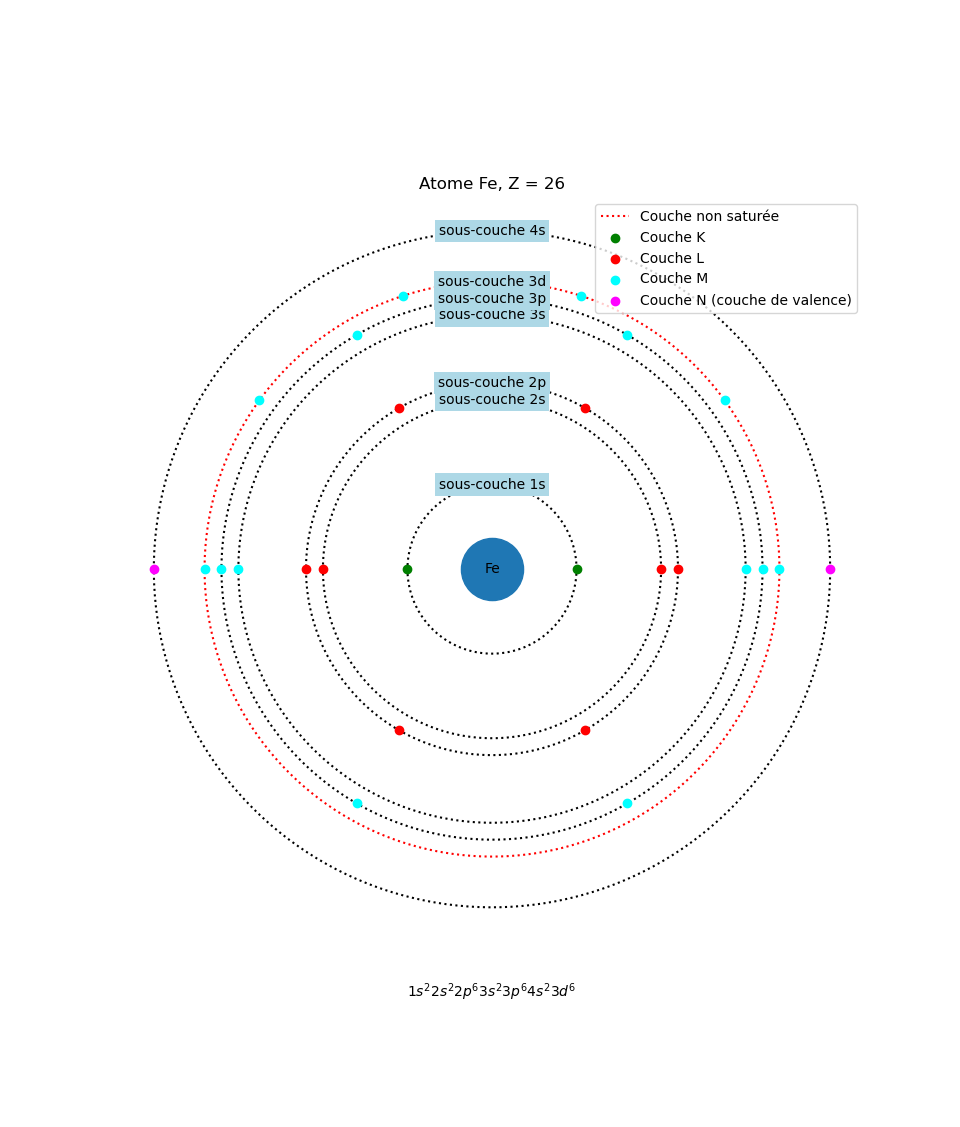
\includegraphics[width=0.85\textwidth,height=\textheight]{./images/physique/Fe.png}

\raggedright

Sur ce shéma, nous pouvons voir plusieurs choses:

\begin{itemize}
\tightlist
\item
  Tout d'abord, les atomes gravitent en couches autour du noyau.
\item
  Les couches sont divisées en sous-couches.
\item
  Les couches et sous-couches ne sont pas remplies dans l'ordre. En
  effet, si nous regardons le shéma, nous pouvons constater que la
  couche qui n'est pas saturée n'est pas la couche \(N\), mais c'est la
  dernière sous-couche de la couche \(M\).
\item
  La dernière couche est appelée couche de valence.
\end{itemize}

\subsection{Les couches}\label{les-couches}

Les atomes sont donc composés de couches, qui sont elles-mêmes divisées
en sous-couches.

Mais avant tout, qu'est ce qu'une couche selon le modèle de Bohr ?

Selon le modèle quantique, une couche symbolise un niveau d'énergie
quantifié. Les électrons se trouvant sur une couche possèdent donc le
niveau d'énergie indiqué par la couche. Une couche éloignée du noyau
(comme par exemple la couche \(N\)) représentera un niveau d'énergie
plus grand qu'une couche proche du noyau (comme par exemple la couche
\(K\)).

Chaque couche \(n\) possède un nombre maximum d'électrons \(2n^2\).
Ceux-ci sont répartis entre les sous-couches.

La couche de valence est la dernière couche.

Les sous-couches peuvent accepter un nombre maximum d'électrons. La
première sous-couche est communément appelée \texttt{s} et accepte au
maximum 2 électrons. La \(n\) ième sous-couche peut accepter au maximum
\(2 + 4n\) électrons.

\subsection{Les liaisons chimiques}\label{les-liaisons-chimiques}

Il existe plusieurs types de liaisons entre les atomes, les molécules et
les ions. Parmi ces liaisons, nous allons nous intéresser plus
particulièrement à:

\begin{itemize}
\tightlist
\item
  liaison covalente
\item
  liaison hydrogène
\end{itemize}

\subsubsection{Liaison covalente}\label{liaison-covalente}

Voici deux atomes et leur représentation:

\begin{Shaded}
\begin{Highlighting}[]
\NormalTok{@startuml}

\NormalTok{\textless{}style\textgreater{}}
\NormalTok{note \{}
\NormalTok{    linecolor transparent}
\NormalTok{    backgroundcolor white}
\NormalTok{\}}
\NormalTok{\textless{}/style\textgreater{}}

\NormalTok{note as O}
\NormalTok{    \textless{}img:/home/fitzwilliam/Documents/bachelor/images/physique/O.png\textgreater{}}
\NormalTok{end note}

\NormalTok{note as H}
\NormalTok{    \textless{}img:/home/fitzwilliam/Documents/bachelor/images/physique/H.png\textgreater{}}
\NormalTok{end note}

\NormalTok{O {-}[hidden]r{-}\textgreater{} H}

\NormalTok{@enduml}
\end{Highlighting}
\end{Shaded}

Nous pouvons constater que ces deux atomes ont leur couche de valence
non saturée.

Selon la règle de l'octet (s'appliquant uniquement aux atomes ayant une
deuxième couche, et éventuellement les deux premières sous-couches de la
troisième couche), les atomes vont essayer d'avoir leur couche de
valence saturée pour atteindre un état stable.

Dans notre cas, la règle de l'octet peut s'appliquer à l'atome
d'oxygène, car celui-ci possède 2 couches, mais pas à l'atome
d'hydrogène.

Cependant, l'atome d'hydrogène va également essayer de saturer sa couche
de valence pour arriver dans un état stable.

Chaque atome d'hydrogène va donc chercher un électron suplémentaire, et
l'atome d'oxygène va chercher 2 électrons suplémentaires (en effet sa
couche de valence ne contient que 4 électrons alors que pour être
saturée, celle-ci doit en contenir 6\ldots)

La solution à ce problème est la liaison covalente: chaque atome
d'hydrogène va partager son électron avec l'atome d'oxygène, et l'atome
d'oxygène va partager un électron avec chacun des 2 atomes d'hydrogène.
Ainsi, grâce à ce partage d'électrons, chacun des atomes a sa couche de
valence saturé et est donc dans un état stable ! Les électrons partagés
entre 2 atomes gravitent autour des 2 atomes, les liant entre eux par
une liaison covalente. Ces liaisons covalentes créent une nouvelle
molécule, la molécule de l'eau \(H_{2}O\). En effet, comme chacun des
atomes a atteint un état stable par le partage d'électrons, aucun ne
voudra partir pour se retrouver à nouveau dans un état pas
stable\ldots{} (Pour changer la molécule, il faut faire des réactions
chimiques)

\subsubsection{Liaison hydrogène}\label{liaison-hydroguxe8ne}

Nous allons reprendre notre molécule d'eau et voir comment les liaisons
hydrogène s'appliquent pour notre molécule.

La molécule est donc composée de plusieurs atomes liés entre eux par des
liaisons covalentes. Cependant, nous avons également vu que les atomes
sont composés de charges positives (dans le noyau), et de charges
négatives (les électrons gravitant autour du noyau). L'électronégativité
d'un atome est donc une grandeur relative qui traduit l'aptitude de cet
atome à attirer vers lui le doublon d'électron liant obtenu par la
liaison covalente. Si l'électronégativité des deux atomes est
différente, la liaison entre les deux atomes est polarisée: un dipôle
électrique est créé (un dipôle électrique est composé d'une charge
positive et d'une charge négative séparé par une distance fixée). Une
molécule peut avoir plusieurs liaisons covalentes polarisées.

Dans le cas de l'oxygène et l'hydrogène, l'oxygène est très
électronégatif, plus que l'hydrogène. Donc les liaisons covalentes
seront polarisées.

Voici l'exemple de la polarisation de la molécule d'eau \(H_{2}O\):

\begin{figure}[H]

{\centering 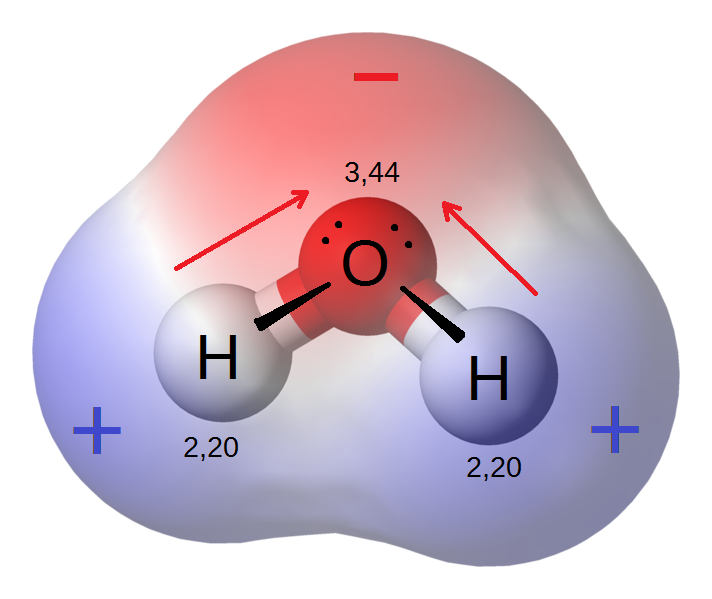
\includegraphics{./images/physique/dipole.png}

}

\caption{Image créée par Riccardo Rovinetti}

\end{figure}%

Dans le graphique, nous pouvons constater 2 flèches. Ces 2 flèches sont
le moment dipolaire de chacune des liaisons covalentes polaires, orienté
du pôle - vers le pôle +. Les nombres indiquent l'électronégativité de
chacun des atomes.

Une liaison hydrogène se produit lorsqu'un atome d'hydrogène lié à un
atome très électronégatif interagit avec un autre atome également très
électronégatif et porteur d'un doublet d'électrons non liant. C'est une
force intermoléculaire moins forte que la liaison covalente.

Dans le cas des molécules d'eau, l'oxygène est très électronégatif. De
plus, l'oxygène partage 2 électrons, donc possède sur sa 2ème couche 2
électrons non liant. Et l'oxygène est lié à l'hydrogène par des liaisons
covalentes polarisées.

Donc lorsqu'on met plusieurs molécules d'eau ensemble, des liaisons
hydrogènes se produisent entre les molécules d'eau.

Les molécules d'eau sont donc maintenues ensembles par une force
intermoléculaire. Si une molécule d'eau est en mouvement, elle aura une
influence sur les autres molécules d'eau avoisinant à cause de ces
liaisons hydrogènes.

\section{Méthode SPH}\label{muxe9thode-sph}

C'est à cet instant qu'intervient la méthode de simulation de fluides
SPH (Smoothed Particle Hydrodynamics).

Cette méthode représente un fluide comme un ensemble de particules.
Chaque particule possède une influence sur les autres particules.

Cette méthode est basée sur une méthode lagrangienne sans maillage.
Différents paramètres physiques sont ajustables.

Nous pouvons constater que cette méthode est assez proche de la réalité,
étant donné les considérations précédentes.

\subsection{\texorpdfstring{La règle de l'octet et la molécule
\(H_{2}O\)}{La règle de l'octet et la molécule H\_\{2\}O}}\label{la-ruxe8gle-de-loctet-et-la-moluxe9cule-h_2o}

La règle de l'octet s'applique uniquement aux atomes appartenant au
groupe principal (les atomes du groupe principal possèdent au plus 3
couches avec uniquement la sous-couche s et p de la couche 3), qui
possèdent un numéro atomique supérieur ou égal à 4.

Cette règle stipule que les électrons des sous-couches \texttt{s} et
\texttt{p} (\texttt{p} est le nom de la \(2^e\) sous-couche) vont
essayer de se combiner pour arriver à 8 électrons. Cela leur permet
d'avoir une configuration stable.

Prenons l'exemple de l'atome d'oxygène (O, Z = 8). Nous pouvons voir sur
le shéma que celui-ci ne possède que 4 électrons dans la couche 2p.
Comme l'oxygène appartient au groupe principal et possède un numéro
atomique supérieur ou égal à 4, la règle de l'octet peut s'appliquer.

La combinaison de la couche 2s et 2p nous donne seulement 6 électrons.
L'atome d'oxygène va donc tenter de récupérer 2 électrons pour arriver à
un état stable.

L'atome d'hydrogène (H, Z = 1) ne possède qu'une seule charge positive.
Pour être dans un état stable, celui-ci va essayer de saturer sa couche
de valence, donc d'acquérir un électron.

Ainsi, l'atome d'oxygène va essayer de récupérer 2 électrons et l'atome
d'hydrogène va essayer de récupérer 1 électron. L'atome d'hydrogène va
donc partager son électron avec l'atome d'oxygène, qui va faire la même
chose: ainsi, l'atome d'oxygène possède un de ses électrons gravitant
autour de l'hydrogène et de lui-même (comme cela l'hydrogène est dans un
état stable), et l'électron de l'atome d'hydrogène gravite également
autour de l'oxygène. Ainsi, l'hydrogène, en partageant son électron, est
dans un état stable. S'il y a un deuxième atome d'hydrogène, les deux
atomes d'hydrogènes sont dans un état stable car l'atome d'oxygène
partage avec eux des électrons, et l'atome d'oxygène est également dans
un état stable car chaque atome d'hydrogène partage avec lui un
électron.

Comme chacun des atomes possède sa couche de valence saturée, il est
heureux et ne voit aucune raison de partir pour se retrouver dans un
état non stable. Les atomes restent donc groupés, liés entre eux par les
partages d'électrons.

Cela forme la molécule d'eau \(H_{2}O\).

\subsection{Liaisons chimiques}\label{liaisons-chimiques}

Il existe plusieurs liaisons entre les molécules.

\begin{itemize}
\tightlist
\item
  Les liaisons fortes: elles sont responsables de la matière solide.
\item
  Les liaisons faibles: elles sont responsables de la matière liquide.
\end{itemize}

\subsection{Méthode SPH (Smooth Particle
Hydro}\label{muxe9thode-sph-smooth-particle-hydro}


\printbibliography


\end{document}
